\section{Theory}
The experiment is based on the phenomenon of multi-beam  from a parallel glass slab. Consider a beam of light falling on a glass slab with refractive index $n$. This beam will undergo multiple refractions and internal reflections inside the slab, as shown below.

The higher order reflections become important if the reflection coefficient $r$ is not very small. $t$ denotes the fraction of amplitude transmitted on entering the slab and $t'$ denotes the fraction transmitted when leaving the slab.
\begin{figure}[H]
  \centering 
  

% Gradient Info
  
\tikzset {_26yuz05ol/.code = {\pgfsetadditionalshadetransform{ \pgftransformshift{\pgfpoint{0 bp } { 0 bp }  }  \pgftransformrotate{0 }  \pgftransformscale{2 }  }}}
\pgfdeclarehorizontalshading{_0h6tu1ewh}{150bp}{rgb(0bp)=(0.94,0.98,1);
rgb(37.5bp)=(0.94,0.98,1);
rgb(49.25bp)=(0.8,0.92,1);
rgb(62.5bp)=(0.63,0.86,1);
rgb(100bp)=(0.63,0.86,1)}

% Gradient Info
  
\tikzset {_i4cvyxn0y/.code = {\pgfsetadditionalshadetransform{ \pgftransformshift{\pgfpoint{0 bp } { 0 bp }  }  \pgftransformrotate{0 }  \pgftransformscale{2 }  }}}
\pgfdeclarehorizontalshading{_2wfq3q3ve}{150bp}{rgb(0bp)=(1,1,1);
rgb(37.5bp)=(1,1,1);
rgb(62.5bp)=(0.9,0.9,0.9);
rgb(100bp)=(0.9,0.9,0.9)}
\tikzset{every picture/.style={line width=0.75pt}} %set default line width to 0.75pt        

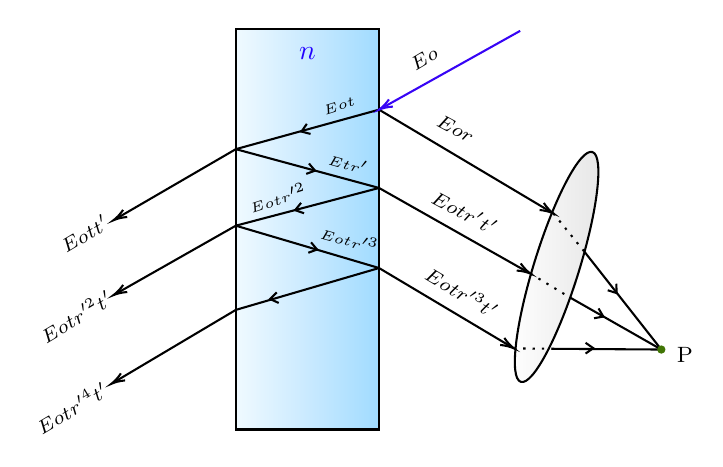
\begin{tikzpicture}[x=0.75pt,y=0.75pt,yscale=-1,xscale=1]
%uncomment if require: \path (0,300); %set diagram left start at 0, and has height of 300

%Shape: Rectangle [id:dp032628939091736475] 
\path  [shading=_0h6tu1ewh,_26yuz05ol] (163,40) -- (232,40) -- (232,233.08) -- (163,233.08) -- cycle ; % for fading 
 \draw   (163,40) -- (232,40) -- (232,233.08) -- (163,233.08) -- cycle ; % for border 

%Shape: Ellipse [id:dp7595942667517073] 
\path  [shading=_2wfq3q3ve,_i4cvyxn0y] (300.31,210.14) .. controls (294.58,208.35) and (297.65,182.12) .. (307.16,151.54) .. controls (316.68,120.96) and (329.05,97.62) .. (334.78,99.41) .. controls (340.51,101.19) and (337.45,127.43) .. (327.93,158) .. controls (318.41,188.58) and (306.05,211.92) .. (300.31,210.14) -- cycle ; % for fading 
 \draw   (300.31,210.14) .. controls (294.58,208.35) and (297.65,182.12) .. (307.16,151.54) .. controls (316.68,120.96) and (329.05,97.62) .. (334.78,99.41) .. controls (340.51,101.19) and (337.45,127.43) .. (327.93,158) .. controls (318.41,188.58) and (306.05,211.92) .. (300.31,210.14) -- cycle ; % for border 

%Straight Lines [id:da885754443074379] 
\draw    (331,147.5) -- (368,194.57) ;
%Straight Lines [id:da8784939845117902] 
\draw    (324,169.5) -- (368,194.57) ;
%Straight Lines [id:da7661126202432749] 
\draw    (315,194.2) -- (368,194.57) ;
%Straight Lines [id:da05051142310491619] 
\draw    (232,79) -- (314.28,127.98) ;
\draw [shift={(316,129)}, rotate = 210.76] [color={rgb, 255:red, 0; green, 0; blue, 0 }  ][line width=0.75]    (6.56,-1.97) .. controls (4.17,-0.84) and (1.99,-0.18) .. (0,0) .. controls (1.99,0.18) and (4.17,0.84) .. (6.56,1.97)   ;
%Straight Lines [id:da6448132052354727] 
\draw    (232,116.72) -- (303.26,157.05) ;
\draw [shift={(305,158.03)}, rotate = 209.51] [color={rgb, 255:red, 0; green, 0; blue, 0 }  ][line width=0.75]    (6.56,-1.97) .. controls (4.17,-0.84) and (1.99,-0.18) .. (0,0) .. controls (1.99,0.18) and (4.17,0.84) .. (6.56,1.97)   ;
%Straight Lines [id:da7382734603266705] 
\draw    (232,155.3) -- (295.28,193.01) ;
\draw [shift={(297,194.03)}, rotate = 210.79] [color={rgb, 255:red, 0; green, 0; blue, 0 }  ][line width=0.75]    (6.56,-1.97) .. controls (4.17,-0.84) and (1.99,-0.18) .. (0,0) .. controls (1.99,0.18) and (4.17,0.84) .. (6.56,1.97)   ;
%Straight Lines [id:da8438722714821767] 
\draw    (232,79) -- (163,98.03) ;
%Straight Lines [id:da6663758152395277] 
\draw    (232,116.72) -- (163,134.9) ;
%Straight Lines [id:da2878880139789143] 
\draw    (232,155.3) -- (163,175.47) ;
%Straight Lines [id:da679672018990835] 
\draw    (163,98.03) -- (105.73,131.3) ;
\draw [shift={(104,132.3)}, rotate = 329.85] [color={rgb, 255:red, 0; green, 0; blue, 0 }  ][line width=0.75]    (6.56,-1.97) .. controls (4.17,-0.84) and (1.99,-0.18) .. (0,0) .. controls (1.99,0.18) and (4.17,0.84) .. (6.56,1.97)   ;
%Straight Lines [id:da5885400756871793] 
\draw    (163,134.9) -- (105.74,167.4) ;
\draw [shift={(104,168.38)}, rotate = 330.42] [color={rgb, 255:red, 0; green, 0; blue, 0 }  ][line width=0.75]    (6.56,-1.97) .. controls (4.17,-0.84) and (1.99,-0.18) .. (0,0) .. controls (1.99,0.18) and (4.17,0.84) .. (6.56,1.97)   ;
%Straight Lines [id:da9028663597097684] 
\draw    (163,175.47) -- (104.72,210.08) ;
\draw [shift={(103,211.1)}, rotate = 329.29] [color={rgb, 255:red, 0; green, 0; blue, 0 }  ][line width=0.75]    (6.56,-1.97) .. controls (4.17,-0.84) and (1.99,-0.18) .. (0,0) .. controls (1.99,0.18) and (4.17,0.84) .. (6.56,1.97)   ;
%Straight Lines [id:da3067635211422284] 
\draw    (232,155.3) -- (163,134.9) ;
%Straight Lines [id:da28570828653091085] 
\draw    (232,116.72) -- (163,98.03) ;
%Straight Lines [id:da9377771078790403] 
\draw [color={rgb, 255:red, 55; green, 4; blue, 245 }  ,draw opacity=1 ]   (300,41.03) -- (233.75,78.03) ;
\draw [shift={(232,79)}, rotate = 330.82] [color={rgb, 255:red, 55; green, 4; blue, 245 }  ,draw opacity=1 ][line width=0.75]    (6.56,-1.97) .. controls (4.17,-0.84) and (1.99,-0.18) .. (0,0) .. controls (1.99,0.18) and (4.17,0.84) .. (6.56,1.97)   ;
\draw   (183.65,172.13) -- (179.54,170.24) -- (182.73,167.03) ;
\draw   (195.86,128.9) -- (191.58,127.42) -- (194.43,123.91) ;
\draw   (199,90.7) -- (194.63,89.55) -- (197.2,85.84) ;
\draw   (199.24,142.93) -- (202.15,146.39) -- (197.91,147.94) ;
\draw   (198.24,104.93) -- (201.15,108.39) -- (196.91,109.94) ;
\draw   (346.3,162.87) -- (346.49,167.38) -- (342.18,166.01) ;
\draw   (337.76,174.78) -- (340.05,178.68) -- (335.6,179.49) ;
%Straight Lines [id:da2986310493998955] 
\draw  [dash pattern={on 0.84pt off 2.51pt}]  (316,129) -- (331,147.5) ;
%Straight Lines [id:da6700491570854924] 
\draw  [dash pattern={on 0.84pt off 2.51pt}]  (305,158.03) -- (324,169.5) ;
%Straight Lines [id:da922121143131131] 
\draw  [dash pattern={on 0.84pt off 2.51pt}]  (297,194.03) -- (315,194.2) ;
\draw   (331.51,191.32) -- (335.22,193.91) -- (331.51,196.5) ;
%Shape: Circle [id:dp01647618202213541] 
\draw  [draw opacity=0][fill={rgb, 255:red, 65; green, 117; blue, 5 }  ,fill opacity=1 ] (366,194.57) .. controls (366,193.46) and (366.9,192.57) .. (368,192.57) .. controls (369.1,192.57) and (370,193.46) .. (370,194.57) .. controls (370,195.67) and (369.1,196.57) .. (368,196.57) .. controls (366.9,196.57) and (366,195.67) .. (366,194.57) -- cycle ;

% Text Node
\draw (192,47.4) node [anchor=north west][inner sep=0.75pt]  [color={rgb, 255:red, 34; green, 1; blue, 255 }  ,opacity=1 ]  {$n$};
% Text Node
\draw (202.74,76.34) node [anchor=north west][inner sep=0.75pt]  [font=\tiny,rotate=-342.63]  {$E\tund{o} t$};
% Text Node
\draw (207.85,97.22) node [anchor=north west][inner sep=0.75pt]  [font=\tiny,rotate=-15.79]  {$E\tund tr'$};
% Text Node
\draw (166.71,121.46) node [anchor=north west][inner sep=0.75pt]  [font=\tiny,rotate=-342]  {$E\tund{o} tr^{\prime 2}$};
% Text Node
\draw (204.08,132.38) node [anchor=north west][inner sep=0.75pt]  [font=\tiny,rotate=-15.8]  {$E\tund{o} tr^{\prime 3}$};
% Text Node
\draw (244.21,54.39) node [anchor=north west][inner sep=0.75pt]  [font=\scriptsize,rotate=-329.1]  {$E\tund{o}$};
% Text Node
\draw (261.51,78.89) node [anchor=north west][inner sep=0.75pt]  [font=\scriptsize,rotate=-28.22]  {$E\tund{o} r$};
% Text Node
\draw (259.51,114.89) node [anchor=north west][inner sep=0.75pt]  [font=\scriptsize,rotate=-28.22]  {$E\tund{o} tr't'$};
% Text Node
\draw (257.12,151.34) node [anchor=north west][inner sep=0.75pt]  [font=\scriptsize,rotate=-30.91]  {$E\tund{o} tr^{\prime 3} t'$};
% Text Node
\draw (75.21,141.39) node [anchor=north west][inner sep=0.75pt]  [font=\scriptsize,rotate=-329.1]  {$E\tund{o} tt'$};
% Text Node
\draw (65.21,184.39) node [anchor=north west][inner sep=0.75pt]  [font=\scriptsize,rotate=-329.1]  {$E\tund{o} tr^{\prime 2} t'$};
% Text Node
\draw (63.21,228.39) node [anchor=north west][inner sep=0.75pt]  [font=\scriptsize,rotate=-329.1]  {$E\tund{o} tr^{\prime 4} t'$};
% Text Node
\draw (374,192.18) node [anchor=north west][inner sep=0.75pt]  [font=\footnotesize] [align=left] {P};


\end{tikzpicture}

  \caption{Multibeam Interference from a parallel slab}
\end{figure}
\noindent
Consider the parallel reflected rays, each of which bears a fixed phase relation with the other. These rays are mutually coherent and will interfere when brought to focus at $P$. Suppose that the incident wave is given by $E\tund{0}e^{i\omega t}$, then the optical field at $P$ is given by:
\begin{align}
    \begin{split}
        \widetilde{E}\tund{1r}&=E\tund{0}r e^{i\omega t}\\ 
         \widetilde{E}\tund{1r}&=E\tund{0}r' t t' e^{i(\omega t-\delta)}\\ 
          \widetilde{E}\tund{1r}&=E\tund{0}r'^3 tt' e^{i(\omega t-2\delta)}\\ 
         & \qquad \vdots\\
           \widetilde{E}\tund{1r}&=E\tund{0}r'^{(2N-3)} tt' e^{i(\omega t-(N-1)\delta)}\\ 
    \end{split}
\end{align}
The total reflected field is equal to the sum of these components, which gives us 
\begin{align}
    \begin{split}
        \widetilde{E}\tund{r} &= \widetilde{E}\tund{1r}+\widetilde{E}\tund{2r}+\ldots+ \widetilde{E}\tund{Nr}\\
        &=E\tund{0}e^{-i\omega t}\qty[r + r'tt' e^{-i\delta}\qty(1 + r'^2 e^{-i\delta}+\ldots+ \qty(r'^2e^{-i\delta})^{N-2})]
    \end{split}
\end{align}
For $\abs{r'^2}<1$ and $N\to \infty$, the above sum becomes an infinite GP and we obtain,  
\begin{align}
    \widetilde{E}\tund{r} = E\tund{0}e^{i\omega t}\qty[r + \frac{r'tt'e^{-i\delta}}{1-r'^2e^{-i\delta}}]
\end{align}
We know that $r'= -r$ and $tt'+r^2=1$, from which we get 
\begin{align}
     \widetilde{E}\tund{r} = \qty[ \frac{1-e^{-i\delta}}{1-r^2e^{-i\delta}}]E\tund{0}e^{i\omega t}r
\end{align}
The reflected flux density at $P$ can be defined as,
\begin{align}
    \mathcal{I}\tund{r}^{\text{\tiny P}} = \frac{1}{2}\widetilde{E}\tund{r}\widetilde{E}\tund{r}^* = \frac{1}{2}E\tund{0}^2\frac{2r^2(1-\cos\delta)}{(1+r^4-2r^2\cos\delta)} =  \frac{\mathcal{F}\sin^2\qty(\delta/2)}{1+\mathcal{F}\sin^2\qty(\delta/2)}\mathcal{I}_i
\end{align}
where $\mathcal{I}_i$ is the incident flux and $\mathcal{F}=\qty(\frac{2r}{1-r^2})^2$ is defined as the \textit{coefficient of finesse}. Similarly for transmitted waves we have, 
\begin{align}
    \widetilde{E}\tund{t} = E\tund{0}e^{i\omega t}\frac{tt'}{1-r^2e^{-i\delta}} \implies  \mathcal{I}\tund{t}^{\text{\tiny P}} = \frac{1}{1+\mathcal{F}\sin^2(\delta/2)}\mathcal{I}_i
\end{align}
From this we can observe that $\mathcal{I}\tund{i} = \mathcal{I}\tund{r}+\mathcal{I}\tund{t}$. Maximum transmission intensity occurs when $\sin(\delta/2)=0\implies \delta\tund{M}=2\pi M$ for integral values of $M$ while minimum intensity occurs when $\sin(\delta/2)=1\implies \delta\tund{m}=(2m+1)\pi$. The maximum and minimum values of intensity are respectively, 
\begin{align}
    \mathcal{I}\tund{t}^{\text{\tiny max}} = \mathcal{I}\tund{i} \qquad \qquad \mathcal{I}\tund{t}^{\text{\tiny min}} =\qty(\frac{1-r^2}{1+r^2})^2 \mathcal{I}\tund{i}
\end{align}
\subsection{Fabry-P\'erot Interferometer}
Having seen the basics of multi-beam interference, we introduce the principle behaind our experimental setup. The Fabry-P\'erot setup constitutes two plane parallel reflecting surfaces within which light rays are multiply reflected and then the transmitted rays are focussed on a screen where they interfere. If we keep the distance between the surfaces fixed, the setup is called an \textit{etalon}. 
\begin{figure}[H]
  \centering 
  

% Pattern Info
 
\tikzset{
pattern size/.store in=\mcSize, 
pattern size = 5pt,
pattern thickness/.store in=\mcThickness, 
pattern thickness = 0.3pt,
pattern radius/.store in=\mcRadius, 
pattern radius = 1pt}
\makeatletter
\pgfutil@ifundefined{pgf@pattern@name@_twufqzfan}{
\pgfdeclarepatternformonly[\mcThickness,\mcSize]{_twufqzfan}
{\pgfqpoint{0pt}{0pt}}
{\pgfpoint{\mcSize+\mcThickness}{\mcSize+\mcThickness}}
{\pgfpoint{\mcSize}{\mcSize}}
{
\pgfsetcolor{\tikz@pattern@color}
\pgfsetlinewidth{\mcThickness}
\pgfpathmoveto{\pgfqpoint{0pt}{0pt}}
\pgfpathlineto{\pgfpoint{\mcSize+\mcThickness}{\mcSize+\mcThickness}}
\pgfusepath{stroke}
}}
\makeatother

% Gradient Info
  
\tikzset {_dxqkoqpuo/.code = {\pgfsetadditionalshadetransform{ \pgftransformshift{\pgfpoint{0 bp } { 0 bp }  }  \pgftransformrotate{0 }  \pgftransformscale{2 }  }}}
\pgfdeclarehorizontalshading{_egreufrhb}{150bp}{rgb(0bp)=(0.96,0.96,0.96);
rgb(37.5bp)=(0.96,0.96,0.96);
rgb(43.821427481515066bp)=(0.86,0.86,0.89);
rgb(57.5bp)=(0.87,0.87,0.89);
rgb(62.5bp)=(0.96,0.96,0.96);
rgb(100bp)=(0.96,0.96,0.96)}
\tikzset{every picture/.style={line width=0.75pt}} %set default line width to 0.75pt        

\begin{tikzpicture}[x=0.75pt,y=0.75pt,yscale=-1,xscale=1]
%uncomment if require: \path (0,300); %set diagram left start at 0, and has height of 300

%Shape: Rectangle [id:dp8328855129785867] 
\draw  [fill={rgb, 255:red, 255; green, 0; blue, 0 }  ,fill opacity=0.9 ] (117,91.37) -- (123,91.37) -- (123,119.37) -- (117,119.37) -- cycle ;
%Shape: Path Data [id:dp20091581139839332] 
\draw  [fill={rgb, 255:red, 248; green, 235; blue, 81 }  ,fill opacity=0.67 ] (340,156) .. controls (339.14,154.26) and (338.35,152.07) .. (337.64,149.53) .. controls (334.27,140.72) and (332,123.87) .. (332,104.53) .. controls (332,86.96) and (333.88,71.44) .. (336.74,62.14) .. controls (337.66,58.47) and (338.74,55.36) .. (340,53) -- (355,53) -- (355,155.75) -- (340,155.75) -- (340,156) -- cycle ;
%Shape: Path Data [id:dp7177299008990078] 
\draw  [fill={rgb, 255:red, 248; green, 235; blue, 81 }  ,fill opacity=0.67 ] (355,53) -- (355,155.75) -- (340,155.75) -- (340,154.13) .. controls (339.66,153.68) and (339.33,153.15) .. (339,152.55) .. controls (334.9,145.06) and (332,126.38) .. (332,104.53) .. controls (332,80.94) and (335.38,61.06) .. (340,54.94) -- (340,53) -- (355,53) -- cycle ;

%Shape: Rectangle [id:dp6806938721428535] 
\draw  [pattern=_twufqzfan,pattern size=11.25pt,pattern thickness=0.75pt,pattern radius=0pt, pattern color={rgb, 255:red, 0; green, 0; blue, 0}] (447,32.95) -- (453,32.95) -- (453,175.47) -- (447,175.47) -- cycle ;
%Shape: Path Data [id:dp33620928543711626] 
\path  [shading=_egreufrhb,_dxqkoqpuo] (243.03,43.21) -- (249.64,43.21) -- (249.78,49.01) -- (288.23,49.01) -- (288.36,43.21) -- (294.97,43.21) -- (302,166.86) -- (285.47,166.86) -- (285.61,161.09) -- (252.38,161.09) -- (252.52,166.86) -- (236,166.86) -- (243.03,43.21) -- cycle (252.24,155.01) -- (285.75,155.01) -- (288.07,55.54) -- (249.93,55.54) -- (252.24,155.01) -- cycle ; % for fading 
 \draw   (243.03,43.21) -- (249.64,43.21) -- (249.78,49.01) -- (288.23,49.01) -- (288.36,43.21) -- (294.97,43.21) -- (302,166.86) -- (285.47,166.86) -- (285.61,161.09) -- (252.38,161.09) -- (252.52,166.86) -- (236,166.86) -- (243.03,43.21) -- cycle (252.24,155.01) -- (285.75,155.01) -- (288.07,55.54) -- (249.93,55.54) -- (252.24,155.01) -- cycle ; % for border 

%Straight Lines [id:da8412820819349593] 
\draw    (123.25,114.03) -- (189.18,143.73) ;
\draw [shift={(191,144.55)}, rotate = 204.25] [color={rgb, 255:red, 0; green, 0; blue, 0 }  ][line width=0.75]    (6.56,-1.97) .. controls (4.17,-0.84) and (1.99,-0.18) .. (0,0) .. controls (1.99,0.18) and (4.17,0.84) .. (6.56,1.97)   ;
%Straight Lines [id:da3791107614020697] 
\draw    (198,145) -- (236.01,140.36) ;
\draw [shift={(238,140.12)}, rotate = 173.04] [color={rgb, 255:red, 0; green, 0; blue, 0 }  ][line width=0.75]    (6.56,-1.97) .. controls (4.17,-0.84) and (1.99,-0.18) .. (0,0) .. controls (1.99,0.18) and (4.17,0.84) .. (6.56,1.97)   ;
%Straight Lines [id:da9637509017276263] 
\draw    (283,131) -- (257.94,124.84) ;
\draw [shift={(256,124.37)}, rotate = 13.8] [color={rgb, 255:red, 0; green, 0; blue, 0 }  ][line width=0.75]    (6.56,-1.97) .. controls (4.17,-0.84) and (1.99,-0.18) .. (0,0) .. controls (1.99,0.18) and (4.17,0.84) .. (6.56,1.97)   ;
%Shape: Path Data [id:dp3529603502503247] 
\draw  [fill={rgb, 255:red, 74; green, 74; blue, 74 }  ,fill opacity=1 ] (255,62.72) -- (255,149.01) -- (252.15,149.01) -- (250.14,62.72) -- (255,62.72) -- cycle ;
%Shape: Path Data [id:dp8486313960010292] 
\draw  [fill={rgb, 255:red, 74; green, 74; blue, 74 }  ,fill opacity=1 ] (283.14,62.72) -- (283.14,149.01) -- (285.99,149.01) -- (288,62.72) -- (283.14,62.72) -- cycle ;
%Straight Lines [id:da9316511896727562] 
\draw    (255,76) -- (279.07,69.5) ;
\draw [shift={(281,68.98)}, rotate = 164.9] [color={rgb, 255:red, 0; green, 0; blue, 0 }  ][line width=0.75]    (6.56,-1.97) .. controls (4.17,-0.84) and (1.99,-0.18) .. (0,0) .. controls (1.99,0.18) and (4.17,0.84) .. (6.56,1.97)   ;
%Straight Lines [id:da8142022442432358] 
\draw    (241,68) -- (221.63,54.15) ;
\draw [shift={(220,52.98)}, rotate = 35.57] [color={rgb, 255:red, 0; green, 0; blue, 0 }  ][line width=0.75]    (6.56,-1.97) .. controls (4.17,-0.84) and (1.99,-0.18) .. (0,0) .. controls (1.99,0.18) and (4.17,0.84) .. (6.56,1.97)   ;
%Straight Lines [id:da6674282070139261] 
\draw    (240,83.65) -- (221.59,69.69) ;
\draw [shift={(220,68.48)}, rotate = 37.17] [color={rgb, 255:red, 0; green, 0; blue, 0 }  ][line width=0.75]    (6.56,-1.97) .. controls (4.17,-0.84) and (1.99,-0.18) .. (0,0) .. controls (1.99,0.18) and (4.17,0.84) .. (6.56,1.97)   ;
%Straight Lines [id:da4633295750425087] 
\draw    (239,99.65) -- (220.59,85.69) ;
\draw [shift={(219,84.48)}, rotate = 37.17] [color={rgb, 255:red, 0; green, 0; blue, 0 }  ][line width=0.75]    (6.56,-1.97) .. controls (4.17,-0.84) and (1.99,-0.18) .. (0,0) .. controls (1.99,0.18) and (4.17,0.84) .. (6.56,1.97)   ;
%Straight Lines [id:da22916627040418092] 
\draw    (239,115.65) -- (220.59,101.69) ;
\draw [shift={(219,100.48)}, rotate = 37.17] [color={rgb, 255:red, 0; green, 0; blue, 0 }  ][line width=0.75]    (6.56,-1.97) .. controls (4.17,-0.84) and (1.99,-0.18) .. (0,0) .. controls (1.99,0.18) and (4.17,0.84) .. (6.56,1.97)   ;
%Straight Lines [id:da8305760719598647] 
\draw    (238,134) -- (219.59,120.04) ;
\draw [shift={(218,118.83)}, rotate = 37.17] [color={rgb, 255:red, 0; green, 0; blue, 0 }  ][line width=0.75]    (6.56,-1.97) .. controls (4.17,-0.84) and (1.99,-0.18) .. (0,0) .. controls (1.99,0.18) and (4.17,0.84) .. (6.56,1.97)   ;
%Straight Lines [id:da22460048854568537] 
\draw    (281,68.98) -- (337.04,57.35) ;
\draw [shift={(339,56.94)}, rotate = 168.27] [color={rgb, 255:red, 0; green, 0; blue, 0 }  ][line width=0.75]    (6.56,-1.97) .. controls (4.17,-0.84) and (1.99,-0.18) .. (0,0) .. controls (1.99,0.18) and (4.17,0.84) .. (6.56,1.97)   ;
%Straight Lines [id:da11775483908577633] 
\draw    (282,82.52) -- (332.03,73.67) ;
\draw [shift={(334,73.32)}, rotate = 169.97] [color={rgb, 255:red, 0; green, 0; blue, 0 }  ][line width=0.75]    (6.56,-1.97) .. controls (4.17,-0.84) and (1.99,-0.18) .. (0,0) .. controls (1.99,0.18) and (4.17,0.84) .. (6.56,1.97)   ;
%Straight Lines [id:da2420787975118045] 
\draw    (283,98.65) -- (331.03,89.68) ;
\draw [shift={(333,89.32)}, rotate = 169.43] [color={rgb, 255:red, 0; green, 0; blue, 0 }  ][line width=0.75]    (6.56,-1.97) .. controls (4.17,-0.84) and (1.99,-0.18) .. (0,0) .. controls (1.99,0.18) and (4.17,0.84) .. (6.56,1.97)   ;
%Straight Lines [id:da6587652898057387] 
\draw    (283,114.65) -- (330.03,105.9) ;
\draw [shift={(332,105.53)}, rotate = 169.46] [color={rgb, 255:red, 0; green, 0; blue, 0 }  ][line width=0.75]    (6.56,-1.97) .. controls (4.17,-0.84) and (1.99,-0.18) .. (0,0) .. controls (1.99,0.18) and (4.17,0.84) .. (6.56,1.97)   ;
%Straight Lines [id:da9849674210877271] 
\draw    (300,127.22) -- (331.04,120.93) ;
\draw [shift={(333,120.53)}, rotate = 168.55] [color={rgb, 255:red, 0; green, 0; blue, 0 }  ][line width=0.75]    (6.56,-1.97) .. controls (4.17,-0.84) and (1.99,-0.18) .. (0,0) .. controls (1.99,0.18) and (4.17,0.84) .. (6.56,1.97)   ;
%Straight Lines [id:da4284319215960505] 
\draw    (355,59.22) -- (446,81.37) ;
%Straight Lines [id:da7827927034228583] 
\draw    (355,116.37) -- (446,81.37) ;
%Straight Lines [id:da6631185675556424] 
\draw    (355,72.37) -- (446,81.37) ;
%Straight Lines [id:da10625579214683667] 
\draw    (354,87.37) -- (446,81.37) ;
%Straight Lines [id:da3308735068532389] 
\draw    (354,102.37) -- (446,81.37) ;
%Straight Lines [id:da5406227117898323] 
\draw    (255,76) -- (282,82.52) ;
%Straight Lines [id:da7109832972019617] 
\draw    (255,92) -- (283,98.65) ;
%Straight Lines [id:da006596316607101804] 
\draw    (255,108) -- (283,114.65) ;
%Straight Lines [id:da036772992717800546] 
\draw    (283,114.65) -- (256,124.37) ;
%Straight Lines [id:da09247680704821226] 
\draw    (283,98.65) -- (255,108) ;
%Straight Lines [id:da20200604101055863] 
\draw    (282,82.52) -- (255,92) ;
\draw   (376.79,60.59) -- (380.19,64.58) -- (375.18,66.13) ;
\draw   (375.39,71.29) -- (378.7,74.95) -- (374.49,77.52) ;
\draw   (372.95,82.51) -- (376.72,85.7) -- (372.89,88.81) ;
\draw   (372.05,95.27) -- (376.63,97.1) -- (373.98,101.26) ;
\draw   (375.05,105.26) -- (379.63,107.1) -- (376.97,111.26) ;
%Straight Lines [id:da3518968314154667] 
\draw    (123,110) -- (187.57,127.3) ;
\draw [shift={(189.5,127.82)}, rotate = 195] [color={rgb, 255:red, 0; green, 0; blue, 0 }  ][line width=0.75]    (6.56,-1.97) .. controls (4.17,-0.84) and (1.99,-0.18) .. (0,0) .. controls (1.99,0.18) and (4.17,0.84) .. (6.56,1.97)   ;
%Straight Lines [id:da91428325264046] 
\draw [color={rgb, 255:red, 74; green, 74; blue, 74 }  ,draw opacity=0.87 ] [dash pattern={on 4.5pt off 4.5pt}]  (107,104) -- (470,104.58) ;
%Straight Lines [id:da5908901825678137] 
\draw    (255,176.58) -- (283,176.58) ;
\draw [shift={(283,176.58)}, rotate = 180] [color={rgb, 255:red, 0; green, 0; blue, 0 }  ][line width=0.75]    (0,3.91) -- (0,-3.91)(7.65,-3.43) .. controls (4.86,-1.61) and (2.31,-0.47) .. (0,0) .. controls (2.31,0.47) and (4.86,1.61) .. (7.65,3.43)   ;
\draw [shift={(255,176.58)}, rotate = 0] [color={rgb, 255:red, 0; green, 0; blue, 0 }  ][line width=0.75]    (0,3.91) -- (0,-3.91)(7.65,-3.43) .. controls (4.86,-1.61) and (2.31,-0.47) .. (0,0) .. controls (2.31,0.47) and (4.86,1.61) .. (7.65,3.43)   ;
%Straight Lines [id:da9049577468314097] 
\draw    (283,131) -- (300,127.22) ;
%Straight Lines [id:da22061796162957015] 
\draw    (255,139.2) -- (283,131) ;
%Straight Lines [id:da40436729878837463] 
\draw    (237,146.2) -- (255,139.2) ;
%Straight Lines [id:da1581018273889172] 
\draw    (238,134) -- (252,140.2) ;
%Straight Lines [id:da7668471632213285] 
\draw    (239,115.65) -- (256,124.37) ;
%Straight Lines [id:da7309466395837563] 
\draw    (239,99.65) -- (256,108.37) ;
%Straight Lines [id:da33903646329786086] 
\draw    (240,83.65) -- (256,92.37) ;
%Straight Lines [id:da029186159080042517] 
\draw    (241,67.88) -- (255,76) ;
%Shape: Path Data [id:dp03167430881467992] 
\draw  [color={rgb, 255:red, 0; green, 0; blue, 0 }  ,draw opacity=1 ][fill={rgb, 255:red, 80; green, 227; blue, 194 }  ,fill opacity=0.64 ] (193.73,162.51) -- (193.73,162.33) -- (193.63,161.42) .. controls (193.62,161.4) and (193.62,161.38) .. (193.61,161.36) .. controls (193.54,161.6) and (193.47,161.84) .. (193.4,162.08) -- (193.42,160.63) .. controls (192.2,155.77) and (191.24,149.88) .. (190.53,143.37) .. controls (189.89,140.2) and (189.5,135.75) .. (189.5,130.82) .. controls (189.5,129.4) and (189.53,128.03) .. (189.59,126.71) .. controls (189.34,120.96) and (189.24,115.03) .. (189.28,109.13) .. controls (189.22,100.8) and (189.45,92.42) .. (189.98,84.56) -- (189.86,84.56) .. controls (190.52,73.97) and (191.71,64.24) .. (193.48,56.77) -- (193.71,54.79) -- (193.7,54.3) .. controls (193.72,54.35) and (193.73,54.4) .. (193.75,54.45) -- (194.91,44.44) -- (196.38,57.15) .. controls (198.06,64.01) and (199.17,73.68) .. (199.7,84.56) -- (199.65,84.56) .. controls (200.08,92.29) and (200.21,100.69) .. (200.04,109.13) .. controls (200.46,130.58) and (198.98,151.69) .. (195.6,162.57) -- (195.59,162.12) -- (194.66,170.57) -- (193.74,162.46) .. controls (193.74,162.47) and (193.73,162.49) .. (193.73,162.51) -- cycle ;

% Text Node
\draw (262,181.4) node [anchor=north west][inner sep=0.75pt]    {$d$};
% Text Node
\draw (182,180) node [anchor=north west][inner sep=0.75pt]  [font=\scriptsize] [align=left] {Lens};
% Text Node
\draw (253,23) node [anchor=north west][inner sep=0.75pt]  [font=\scriptsize] [align=left] {Etalon};
% Text Node
\draw (322,162) node [anchor=north west][inner sep=0.75pt]  [font=\scriptsize] [align=left] {\begin{minipage}[lt]{31.68pt}\setlength\topsep{0pt}
Focusing
\begin{center}
 lens
\end{center}

\end{minipage}};
% Text Node
\draw (431,183) node [anchor=north west][inner sep=0.75pt]  [font=\scriptsize] [align=left] {Screen};
% Text Node
\draw (91,127) node [anchor=north west][inner sep=0.75pt]  [font=\scriptsize] [align=left] {\begin{minipage}[lt]{39.21pt}\setlength\topsep{0pt}
\begin{center}
Extended \\light source
\end{center}

\end{minipage}};


\end{tikzpicture}

  \caption{Schematic diagram of the Fabry-Perot experimental set-up}
\end{figure}
\noindent 
Sometimes transparent metal films are used to increase the reflectance $R=r^2$ but introducing this also incurs an absorptance $A$. Along with the transmittance $T$, the conservation equation becomes 
\begin{align}
    R+T+A=1
\end{align}
Another complication due to the metallic film is the introduction of an additional phase $\phi$ which depends on $\theta\tund{i}$ (the angle of the incident rays). The phase difference between the two successively transmitted rays is,
\begin{equation}
    \delta = \frac{4\pi n}{\lambda\tund{0}} d\cos\theta\tund{t}+2\phi
\end{equation}
where $n$ is the refractive index of the plates, $\lambda\tund{0}$ is the wavelength of the light source and $\theta\tund{t}$ is the angle of the transmitted ray. Considering small $d$ and large $\lambda\tund{0}$, we can safely neglect $\phi$. From this, the transmission ratio is given as, 
\begin{align}
   \begin{split}
     \frac{\mathcal{I}\tund{t}}{\mathcal{I}\tund{i}} = \qty(\frac{T}{1-R})^2 \times \qty({1+\frac{4R}{(1-R)^2}\sin^2\qty(\delta/2)})^{-1} &=\qty( \frac{1-R-A}{1-R})^2 \frac{1}{1+\mathcal{F}\sin^2\qty(\delta/2)}\\ &= \qty[1-\frac{A}{1-R}]\qty({1+\mathcal{F}\sin^2\qty(\delta/2)})^{-1}
   \end{split}
\end{align}
\subsection{Sharpness and Finess}
To analyse the sharpness of the peak, we find the half-width $\gamma$, which tells us the characteristic width of the peak. We obtain it by solving for $\delta$ where $\mathcal{I}\tund{t} = \frac{1}{2}(\mathcal{I}\tund{t})\tund{max}$ from which we obtain the condition, 
\begin{equation}
    \begin{split}
        \frac{1}{1+\mathcal{F}\sin^2\qty(\delta/2)} = \frac{1}{2}\implies \sin\qty(\frac{\delta\tund{1/2}}{2}) = \frac{1}{\sqrt{\mathcal{F}}}
    \end{split}
\end{equation}
For large $\mathcal{F}$, the sin term is very small and hence can be approximated as simply $\frac{\delta\tund{1/2}}{2}$ which gives us $\gamma \equiv 2\delta\tund{1/2} = \frac{4}{\sqrt{\mathcal{F}}}$. The ratio of separation of adjacent maxima divided by the half-width is defined as the finesse, $\mathscr{F}$. The difference between maximas is $2\pi (m+1) - 2\pi m = 2\pi$ and hence, 
\begin{equation}
    \mathscr{F} = \frac{2\pi}{\gamma} = \frac{\pi\sqrt{\mathcal{F}}}{2}
\end{equation}
\section{Working Formula}
The intensity of transmitted light will follow the relation, 
\begin{equation}\label{trans}
    \mathcal{T} = \frac{\uptau\tund{0}}{1+\mathcal{F}\sin^2\qty(2\pi L/\lambda)}
\end{equation}
where $\uptau\tund{0}$ is the maximum possible intensity and $L$ is the `optical spacing' between the mirrors that depend on the refractive index, transmittance angle and the spacing $d$ between the mirrors. 
\begin{equation}
    L = 2\pi n d \cos\theta\tund{t}
\end{equation}
The finesse  $\mathscr{F}$ and the contrast $\mathcal{C}$ are defined as,
\begin{equation}
     \mathscr{F}=\frac{\pi\sqrt{\mathcal{F}}}{2} = \frac{\pi r}{1-r^2}\qquad \mathcal{C} = \mathscr{F}+1
\end{equation}
For circular fringes, the fringe radius $\chi\tund{m}$ is related to the $m$-th ring using, 
\begin{equation}\label{radius}
    \chi\tund{m}^2 = \frac{D^2 \lambda}{d} m
\end{equation}
where $D$ is the distance between the etalon and the screen and $d$ is the distance between the mirrors. 